\chapter{Uma Rede de Colaboração para a UnB}

Como já exposto, o objetivo deste trabalho é disponibilizar um ambiente
virtual no qual alunos, professores e servidores técnico-administrativos tenham
um espaço para a criação e o compartilhamento de conhecimento na forma de uma
rede de colaboração livre para a Universidade de Brasília: o Comunidade.UnB.
%
Para isto, escolhemos a plataforma Noosfero por entender que
(\textit{i}) as funcionalidades de rede social e de CMS satisfazem nossas
necessidades; (\textit{ii}) além das vantagens existentes por este ser uma
plataforma de software livre; (\textit{iii}) por ser  expansível (através de
\textit{plugins}); (\textit{iv}) por ter uma comunidade ativa e pela posição
geográfica favorável que possuímos em relação ao núcleo de desenvolvimento
dela, que está no Brasil.
%
Desta forma, conseguimos facilmente contactar os principais desenvolvedores
do Noosfero e organizar encontros para discutir parcerias, como ocorrido
algumas vezes durante este trabalho, tanto presencialmente quanto remotamente.

Além de um ambiente virtual para interação social, queremos que a rede proposta
funcione como um ambiente para os alunos, professores e funcionários da
universidade compartilhar ideias, produzir conteúdo de forma colaborativa e
publicá-lo para que possa ser de utilidade para outras pessoas ou parcelas da
sociedade, uma vez que entendemos (e defendemos) ser este um dos papéis de uma
Universidade: universalizar o conhecimento.
%
O ambiente disponibiliza para seus usuários a capacidade de criar blogs,
comunidades, de se relacionar com outras pessoas e ao mesmo tempo associar seu
perfil à marca da Universidade de Brasília.

As comunidades no Comunidade.UnB podem ser utilizadas para construir e publicar
conteúdo de áreas de conhecimento, disciplinas e projetos acadêmicos de forma
colaborativa, como ocorreu, em nossos estudos de caso, em 3 disciplinas da UnB Gama.
%
Dentre as vantagens dessa abordagem podemos destacar a possibilidade de
acesso do público ao conteúdo, e a continuidade do conteúdo desenvolvido
nas comunidades para outras pessoas que eventualmente se juntem ao longo do tempo.
%
Entretanto, o Noosfero permite configurar a publicação do conteúdo de suas
comunidades, de forma a decidir quais conteúdos serão expostos ao público e
quais seriam mantidos privados.

\begin{figure}[h]
    \centering
    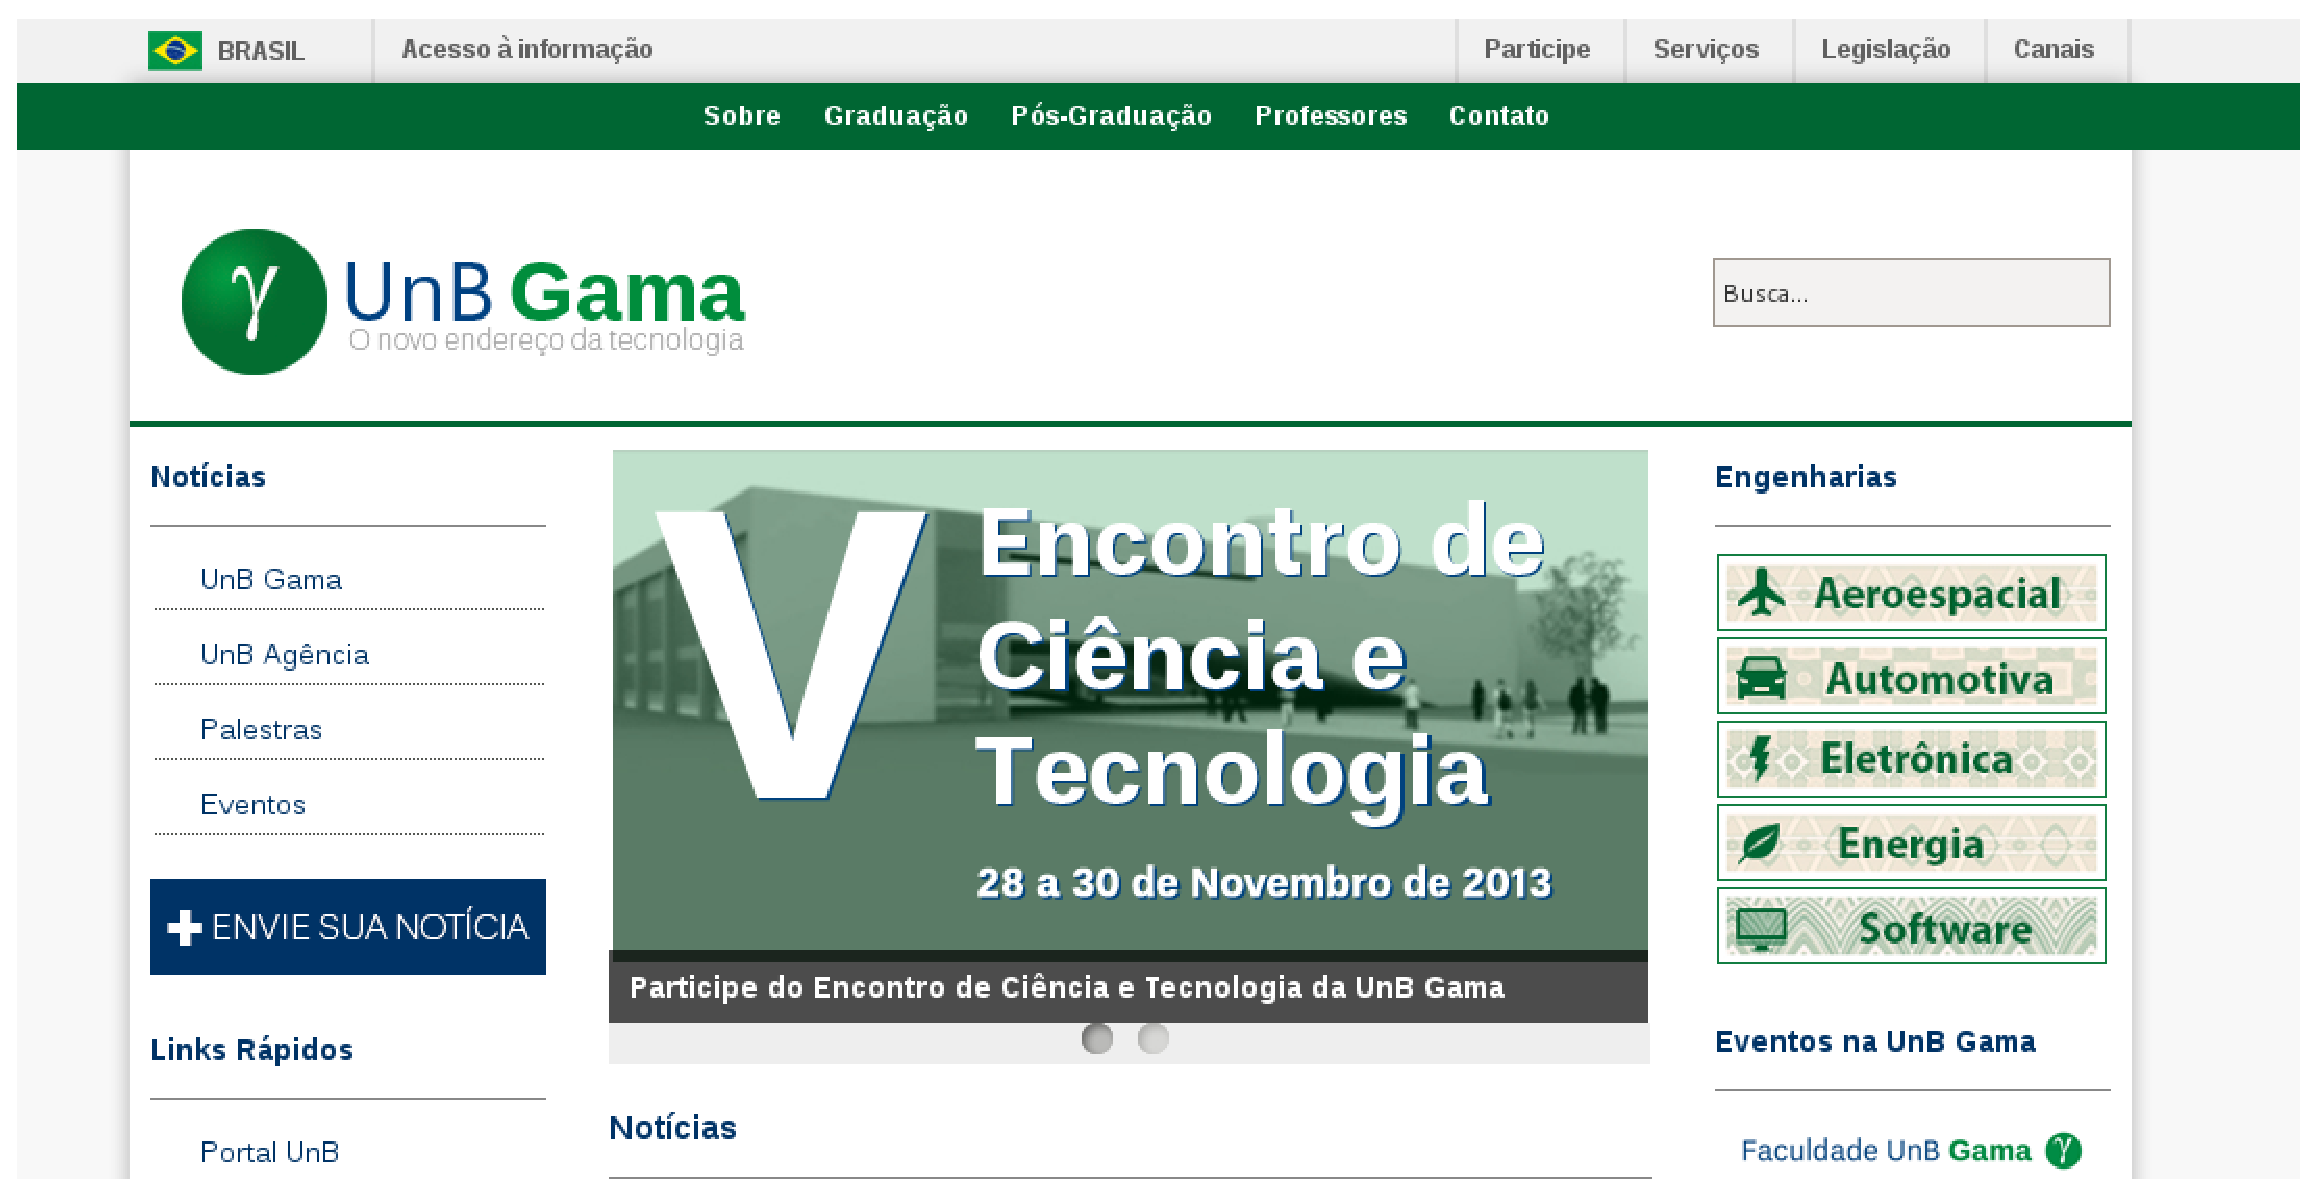
\includegraphics[keepaspectratio=true,scale=0.4]
      {figuras/portal-fga.eps}
    \caption{Ambiente Noosfero como portal da Faculdade do Gama}
    \label{portal-fga}
\end{figure}

O Noosfero permite também fazer uso de suas funcionalidades de CMS para a
criação de portais institucionais para faculdades, departamentos, laboratórios,
dentre outros. A Figura \ref{portal-fga} apresenta o uso de um ambiente
Noosfero como portal para a Faculdade UnB Gama (FGA), que também recebeu
colaborações durante este trabalho, desde o desenvolvimento de funcionalidades com a equipe,
passando pelo treinamento da mesmo, até a revisão de código de contribuições da mesma.
%
No contexto do Portal da FGA, podemos ter comunidades dentro do
Comunidade.UnB com temas próprios que funcionariam como portais institucionais.
%
Em outras palavras, dependendo do o que for planejado para o Comunidade.UnB, o
Portal da FGA pode, no futuro ser, na prática, uma comunidade dentro do Comunidade.UnB,
com os seus respectivos sub-grupos.

Nesse capítulo apresentaremos as funcionalidades desenvolvidas para contribuir
para a adequação do Noosfero como uma rede de colaboração para universidades,
os requisitos não-funcionais levantados para que esta possa suprir as
necessidades de segurança e confiabilidade e o processo de colaboração com o
Noosfero. O capítulo \ref{cap:conclusao}, na seção de trabalhos futuros,
apresenta outras funcionalidades que
foram levantadas por nós mas não foram desenvolvidas ao longo deste trabalho.

%------------------------------------------------------------------------------%
\section{Processo de colaboração para o Noosfero}

Um desafio frequente encontrado em comunidades de software livre, principalmente
comunidades de projetos menores ou novos, é elaborar um processo e utilizar
ferramentas que facilitem e incentivem a entrada de novas pessoas.
\citeonline{reis2003} identificou que 65\% dos projetos de software livre
utilizam ferramentas de controle de versão, listas de correio eletrônico e a
página do projeto na internet como ferramenta de comunicação entre usuários e
desenvolvedores. Hoje, dez anos depois desse levantamento, podemos ter em mente
que esse percentual seja bem maior.
%
Em 2011, uma pesquisa, realizada por \citeonline{corbucci2011}
para sua dissertação de mestrado, identificou listas de correio eletrônico como
sendo a ferramenta de comunicação mais comum em projetos de software livre
seguido pelo \textit{Internet Relay Chat} (IRC).
%
A comunidade do Noosfero faz uso de todas as ferramentas citadas acima, com
o objetivo de minimizar os problemas de comunicação ocasionados pelo fato da
equipe estar distribuída ao redor do mundo, bem como, possibilitar que novos
membros da comunidade, sejam eles desenvolvedores ou usuários, possam se
integrar do que está ocorrendo no projeto e interagir com os demais membros.

As lista de correio eletrônico
~\footnote{\url{https://noosfero.org/Development/MailingLists\#Development}}
(são duas: uma em português, para comunidade brasileira, e outra em inglês,
para os desenvolvedores com um todo, brasileiros ou não) é a principal
ferramenta de comunicação.
%
Além disso, a comunidade mantém um canal no IRC~\footnote{Os canais \#noosfero e
\#noosfero-br hospedados no FreeNode até o momento da escrita deste texto.}
para tirar dúvidas e proporcionar um canal de comunicação mais dinâmica.
%
Outra iniciativa recente da comunidade para melhorar a comunicação e manter os
diversos núcleos de desenvolvimentos do Noosfero a par das últimas atualizações
é a de realizar quinzenalmente reuniões via vídeo-conferência.

A página do Noosfero~\footnote{\url{http://noosfero.org}} possui uma seção de
desenvolvimento~\footnote{\url{http://noosfero.org/Development}} que apresenta
informações necessárias para pessoas que queiram começar a colaborar com o
mesmo. Nessa página, encontramos também um \textit{issue tracker} utilizado para
cadastrar e mapear o desenvolvimento das funcionalidades e correções de
\textit{bugs} do Noosfero.
%
São disponibilizados dois \textit{issue trackers} diferentes, um para
funcionalidades e outro para \textit{bugs}. Ao cadastrar um novo item
(também chamado de \textit{issue} ou \textit{Action Item}), o
desenvolvedor preenche os campos com o título daquele item; uma ou mais
categorias para aquele item (e.g. Chat, RSSFeeds); a descrição daquele
item; o \textit{plugin} relacionado aquele item, quando existir; e a
versão do Noosfero que aquele item afeta.
%
Para funcionalidades, coloca-se a
versão em que essa está prevista para ser lançada, enquanto que para
\textit{bugs}, coloca-se também a versão em que este foi identificado. Com o
item criado, outro usuários podem adicionar comentários e associar um
desenvolvedor responsável pela sua implementação.

\begin{figure}[h]
    \centering
    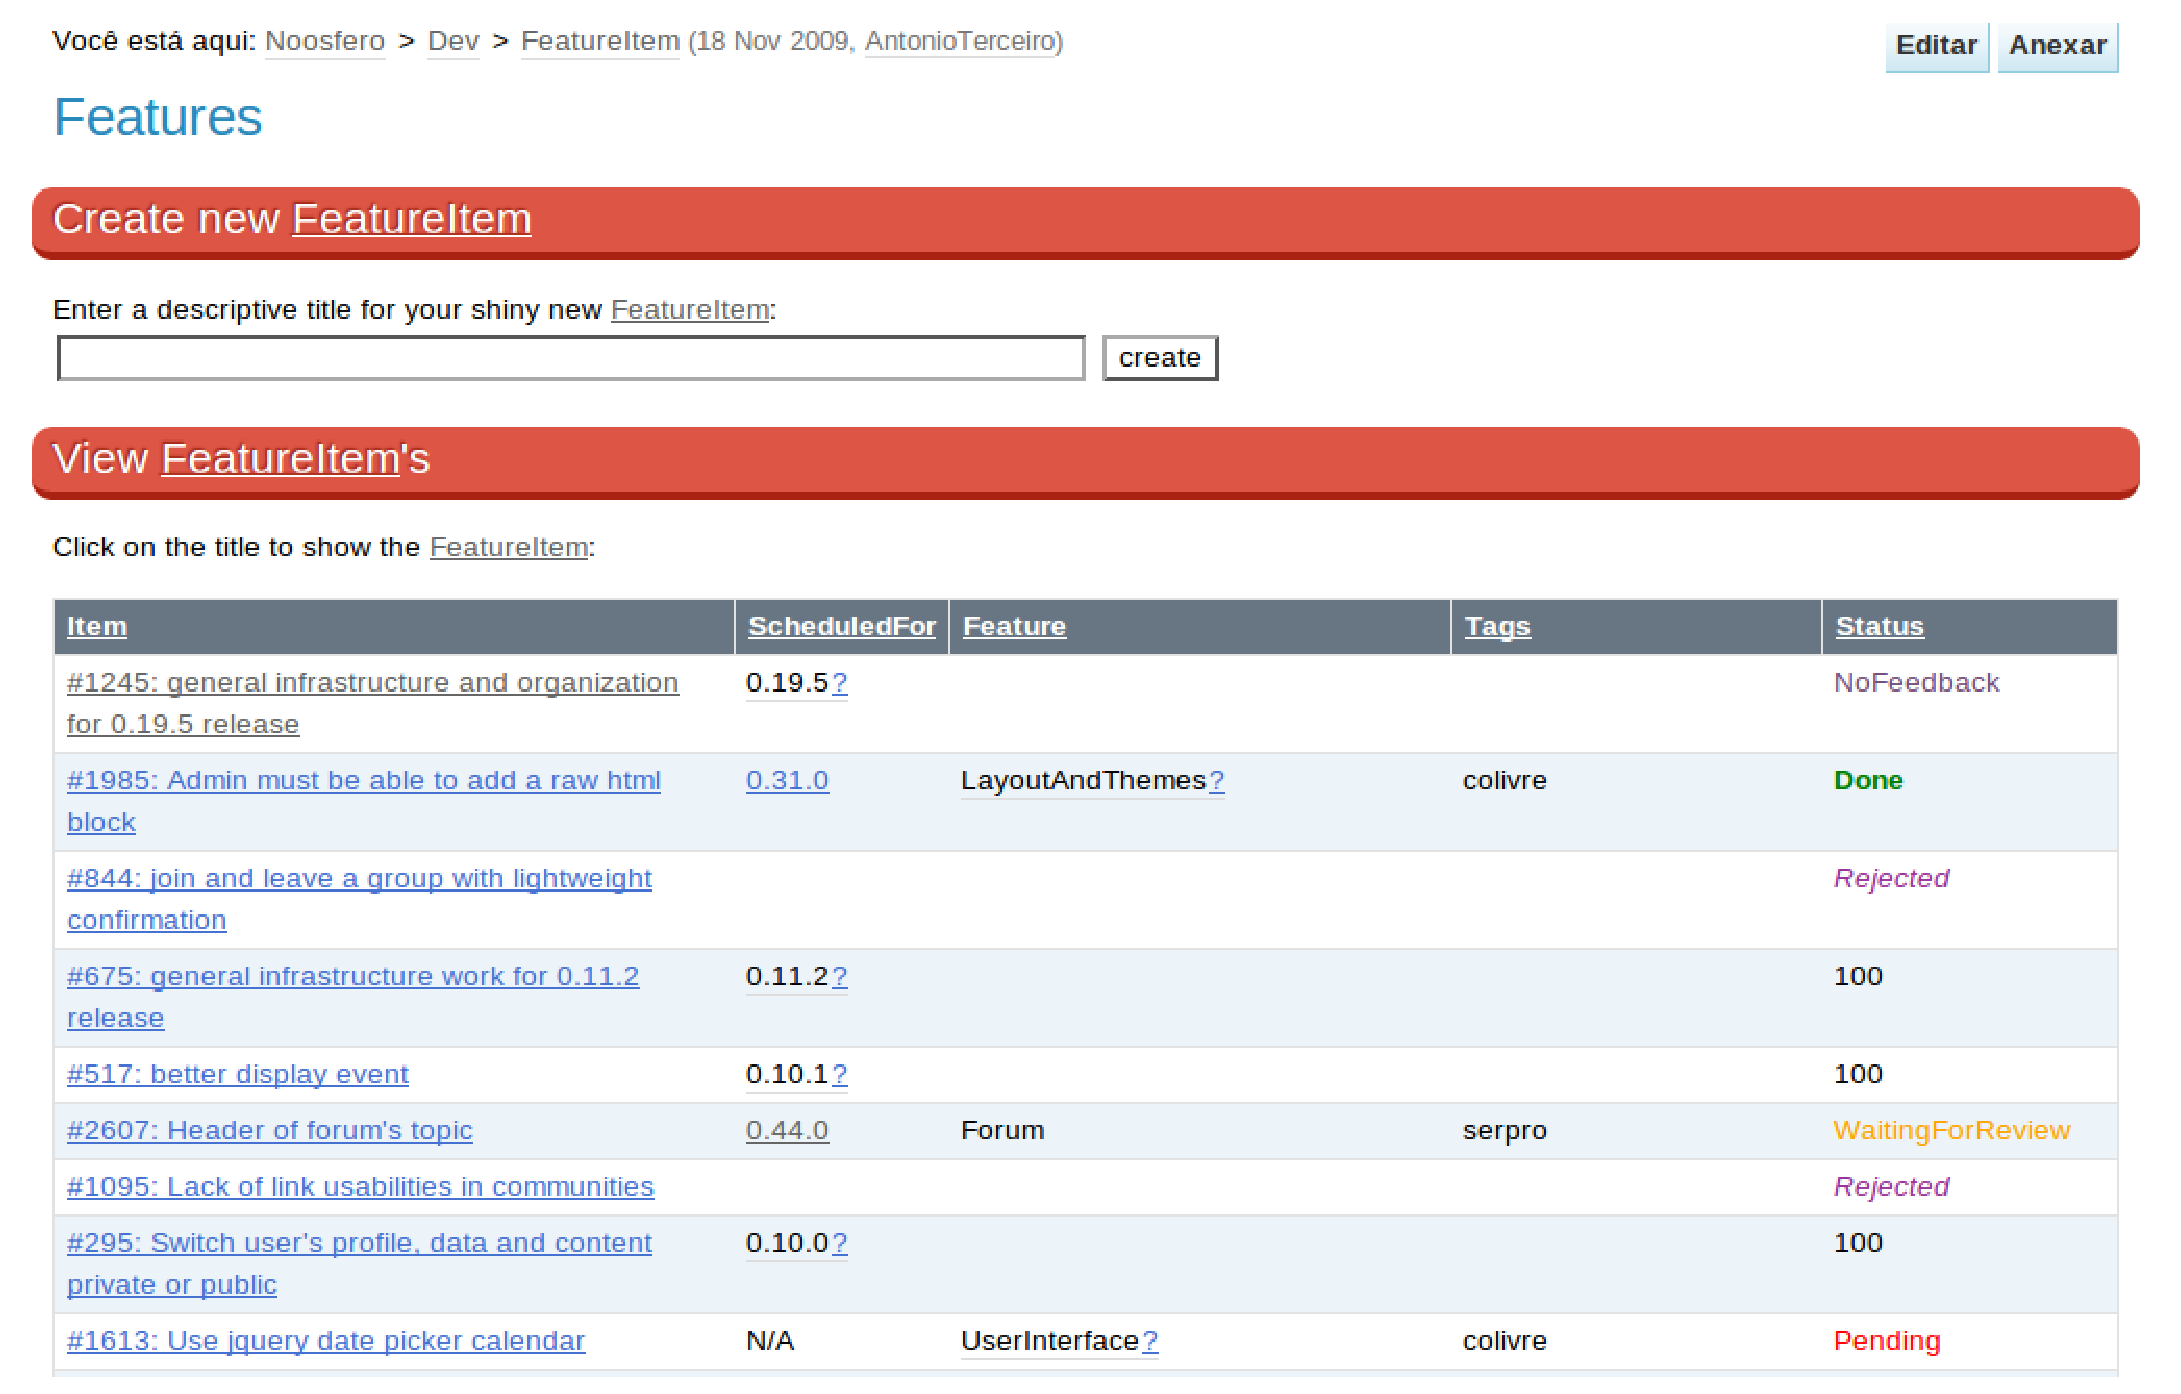
\includegraphics[keepaspectratio=true,scale=0.4]
      {figuras/issue-tracker.eps}
    \caption{Issue Tracker do Noosfero}
    \label{issue-tracker}
\end{figure}

A Figura \ref{issue-tracker} apresenta o \textit{issue tracker} para
funcionalidades do Noosfero.
%
A pessoa que queira cadastrar novos itens nestes precisa se cadastrar
na página de desenvolvimento do Noosfero.
%
Recentemente, foi implementado um sistema que possibilita à comunidade declarar
seu interesse em ver um item resolvido, dessa forma é possível priorizar os
itens identificados como sendo de maior importância para os usuários e
desenvolvedores.

A ferramenta utilizada para controle de versão é o Git~\footnote{
\url{http://git-scm.com/}}, uma ferramenta livre de versionamento distribuído
de código fonte. O repositório oficial do Noosfero encontra-se no Gitorious
~\footnote{\url{https://gitorious.org/noosfero/noosfero}} com um espelho no
Gitlab~\footnote{\url{https://gitlab.com/noosfero/noosfero}} e outro no
Github~\footnote{\url{https://github.com/noosfero/noosfero}}.
%
Na página de desenvolvimento da comunidade existe uma série de recomendações
sobre como enviar \textit{patches} para o Noosfero%
~\footnote{\url{https://noosfero.org/Development/PatchGuidelines}},
desde como versionar seu \textit{patches}, até como realizar a solicitação de
inclusão do seu \textit{patch}, ou \textit{merge-request}, na plataforma.

O processo de colaboração com o Noosfero incluí uma série práticas apresentadas
pelas metodologias ágeis de desenvolvimento de software como o uso de testes
automatizados, a descrição das funcionalidades do projeto no formato de
histórias de usuário e a adoção de ferramentas para a utilização da metodologia
\textit{Behavior Driven Development} (BDD)%
~\footnote{\url{http://en.wikipedia.org/wiki/Behavior-driven_development}},
uma evolução do \textit{Test Driven Development} (TDD)%
~\footnote{\url{http://en.wikipedia.org/wiki/Test-driven_development}}
apresentada por \citeonline{north2006}, como veremos na Seção
\ref{funcionalidades}.
%
As semelhanças das práticas adotadas pelas comunidades de software livre e as
comunidades de métodos ágeis foram apresentadas por \citeonline{corbucci2011}
em sua tese de mestrado. De acordo com ele, os dois
métodos possuem tantas características em comum ao ponto de, Martin Fowler,
um dos autores mais influentes na Literatura sobre métodos ágeis,
incluir software livre como um método ágil na primeira versão de seu artigo
\textit{"The New Methodology"}. No entanto o mesmo foi retirado devido
à falta de descrição precisa dos métodos de desenvolvimento utilizados pelas
comunidades de software livre \apud[p.~9]{fowler2000}{corbucci2011}.
%
Por outro lado, \citeonline{corbucci2011} discute os princípios ágeis e livres
como semelhantes:
%
(\textit{i}) Indivíduos e interações são mais importantes que processos e
ferramentas;
(\textit{ii}) Software em funcionamento é mais importante que documentação
abrangente;
(\textit{iii}) Colaboração com o cliente (usuários) é mais importante que
negociação de contratos;
(\textit{iv}) Responder às mudanças é mais importante que seguir um plano.
%
Também, explicita as práticas disseminadas pelas metodologias ágeis usadas no
cotidiano dos desenvolvedores de software livre:
(\textit{i}) Código compartilhado (coletivo);
(\textit{ii}) Projeto simples;
(\textit{iii}) Repositório único de código;
(\textit{iv}) Integração contínua;
(\textit{v}) Código e teste;
(\textit{vi}) Desenvolvimento dirigido por testes, e
(\textit{vii}) Refatoração~\cite{corbucci2011}. Portanto, neste trabalho,
entendemos software livre com um método ágil de desenvolvimento, do ponto de
vista da Engenharia de Software.

\section{Requisitos Não-funcionais}

Antes dos funcionalidades desenvolvidas (apresentadas na próxima seção),
investigamos os requisitos não-funcionais. Dessa forma, separamos algumas
características que julgamos necessárias para o bom funcionamento do
Comunidade.UnB, principalmente em relação à disponibilidade, performance e
segurança do sistema.

É importante para o sucesso da Comunidade.UnB que ele permaneça disponível
mesmo durante picos de acesso estimados em até 30 mil usuários simultâneos,
que dá aproximadamente 75\% do total de candidatos a usuários da Universidade
que possui atualmente 2.445 professores, 2.630 técnicos-administrativos
e 28.570 alunos regulares e 6.304 de pós-graduação, totalizando de 39.949
\cite{unbInstituicao}. Como explicado na seção \ref{noosfero-section}, o Noosfero
utiliza o \textit{web-server} Apache como um servidor de \textit{proxy} reverso
que realizar o balanceamento de carga entre as diversas instâncias do Thin,
configuradas durante a instalação, sendo que são recomendadas a configuração de
duas instâncias por núcleo de processador presentes na máquina que está
hospedando o sistema.
%
Estimamos que necessitaríamos de 8 instâncias do Thin
para manter um nível de performance aceitável durante picos de acesso, o que
necessitaria de uma máquina com pelo menos 4 núcleos de processamento para
hospedar o sistema. No entanto, essa estimativa foi realizada com base em
depoimentos de usuários destas tecnologias e faz-se necessária a execução de
um \textit{benchmark} mais específico para podermos definir estes parâmetros com
uma precisão maior.
%
Na seção \ref{sec:future-works} propomos um estudo sobre escalabilidade para
aplicações desenvolvidas em \textit{Ruby on Rails} e a possibilidade de se
utilizar mais de uma máquina hospedeira para tanto.

%TODO adquirir certificado SSL em trabalhos futuros
No quesito segurança, é importante que as requisições que chegam ao serviço
do Comunidade.UnB passem por uma camada de criptografia para impedir que
eventuais ataques consigam recuperar dados como a senha do usuário. Assim faz-se
necessário a adição de uma camada de \textit{Secure Socket Layer/Transport
Layer security} (SSL)/TLS através do protocolo \textit{Hypertext Transfer
Protocol Secure} (HTTPS) para acesso à Comunidade.UnB. As permissões de acesso das
comunidades e seu conteúdo podem ser configuradas através do painel de controle
das mesmas. Essa é uma preocupação já bastante discutida na comunidade do
Noosfero e no momento da escrita deste texto esta estava implementando algumas
alterações para adequar o Noosfero ao uso de SSL. Será necessário adquirir um
certificado válido para utilização de SSL no Comunidade.UnB.

\begin{figure}[h]
    \centering
    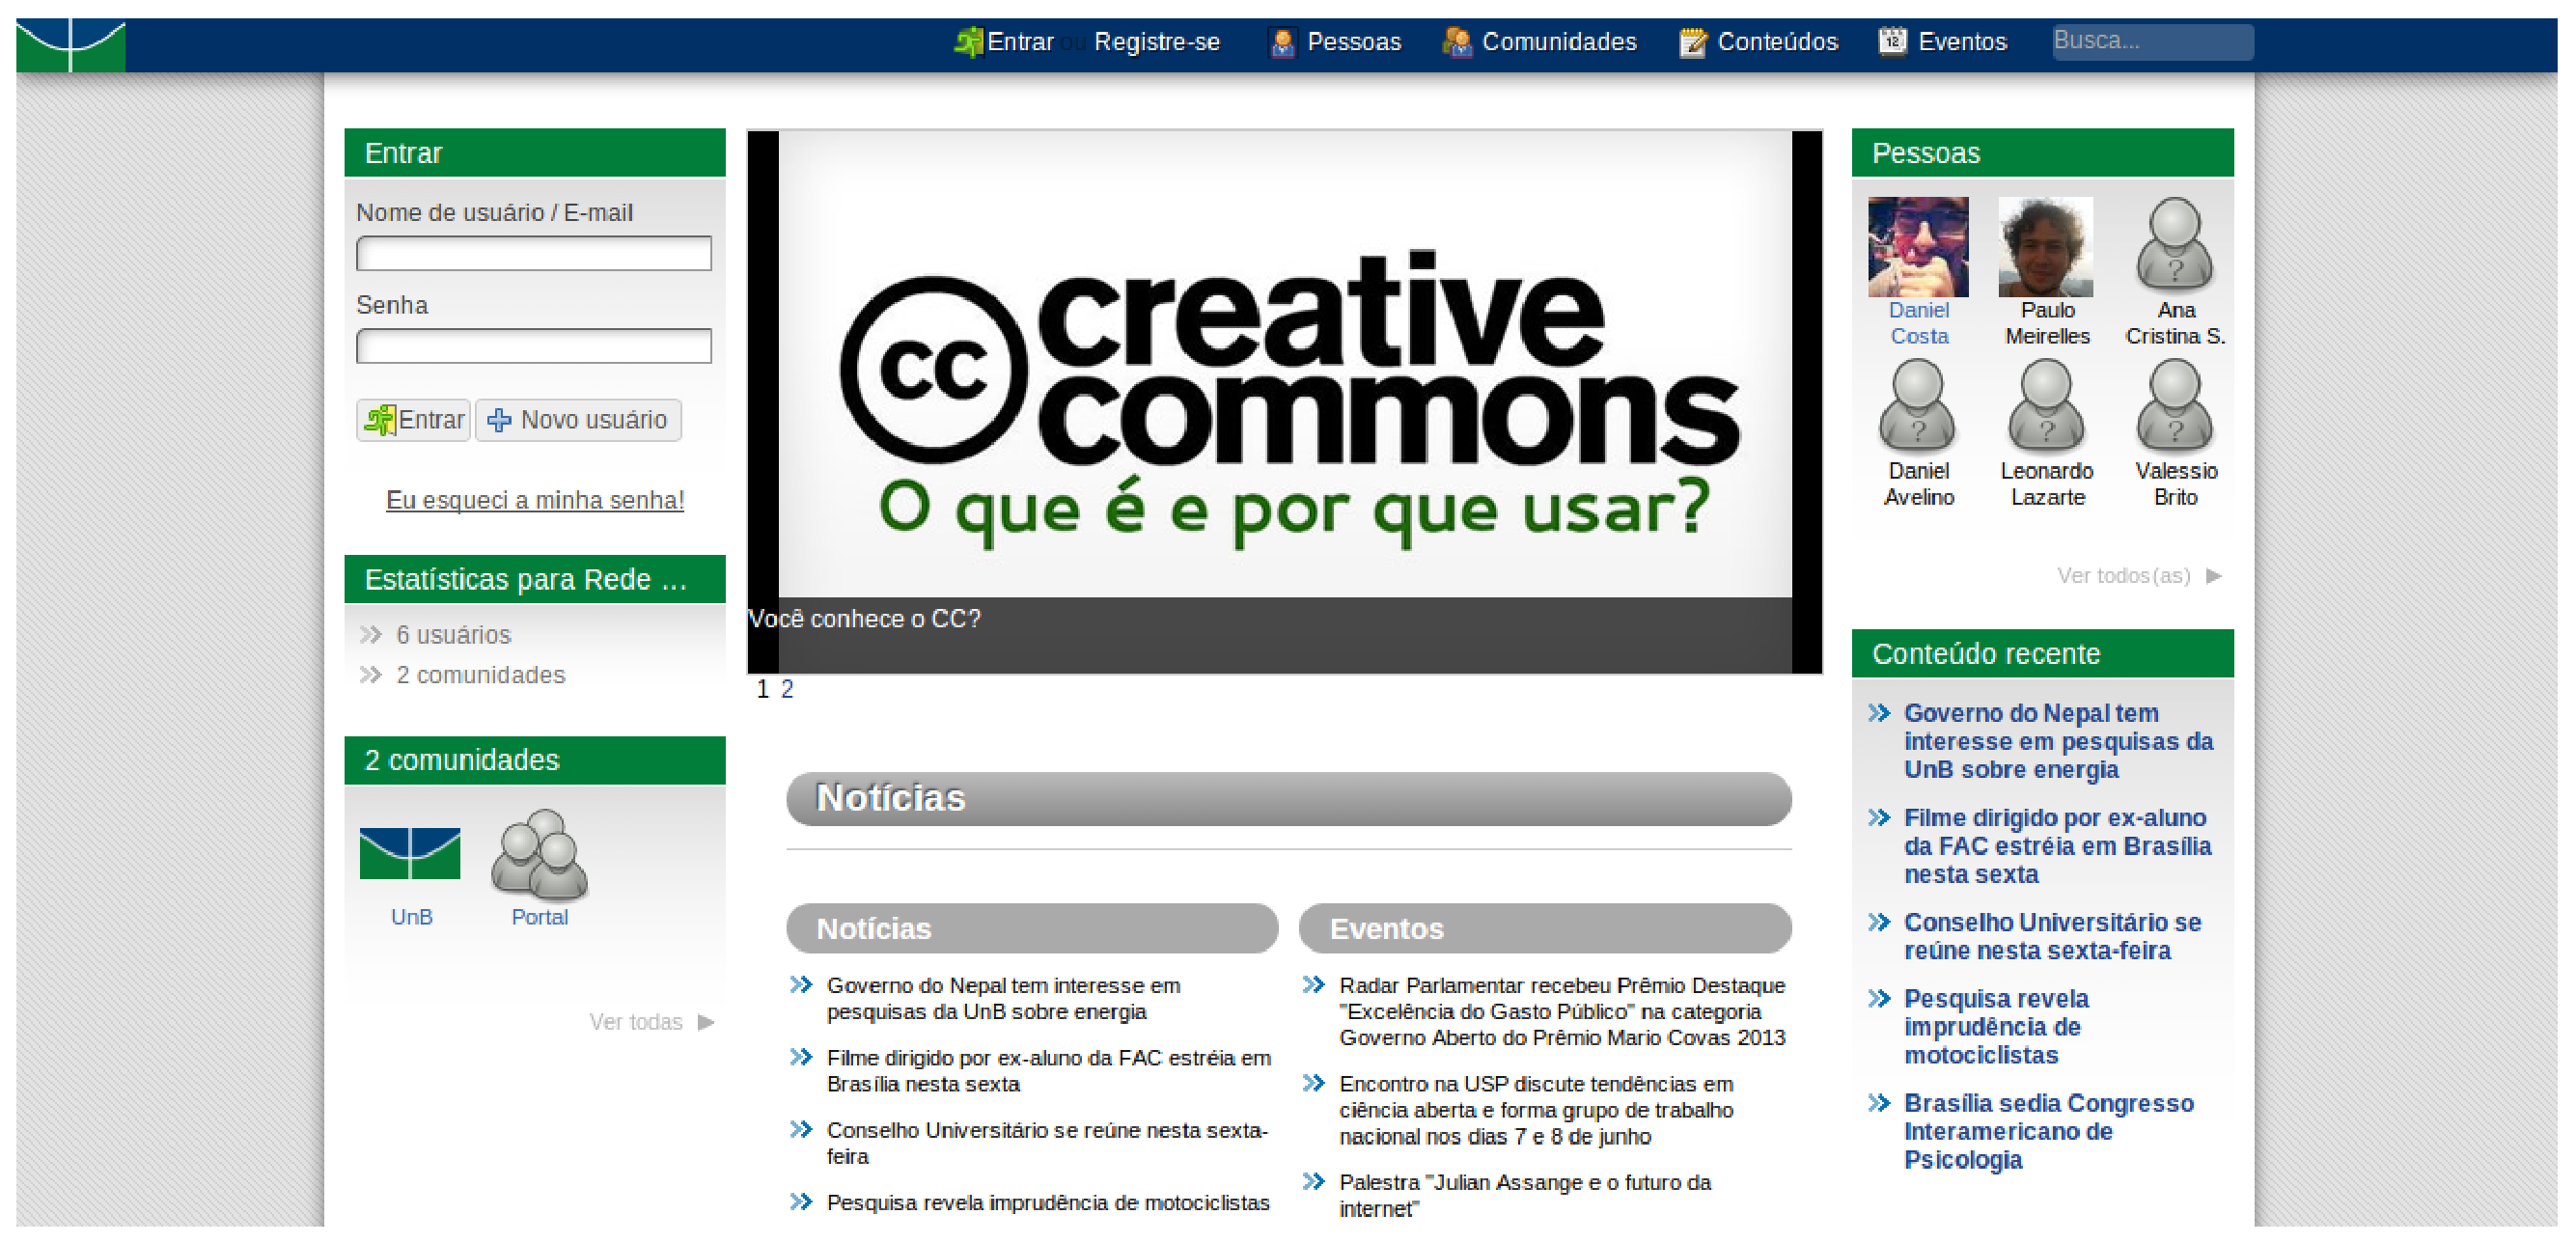
\includegraphics[keepaspectratio=true,scale=0.4]
      {figuras/comunidade.unb.br.eps}
    \caption{Página inicial da Comunidade.UnB}
    \label{comunidade-unb}
\end{figure}

Outro aspecto importante que levamos em consideração é a adequação da
Comunidade.Unb ao padrão de identidade visual da UnB.
A identidade visual da rede foi adaptada em cima do tema~\footnote{Temas são
compostos por aquivos de \textit{layout}, em rhtml e CSS, que definem os aspectos
visuais de uma instância do Noosfero. Os temas podem ser alterados pela interface
administrativa da instância.} do Stoa, que é disponibilizada em um repositório
público, para se enquadrar no padrão da UnB e está disponível em um repositório
no \textit{Github}~\footnote{\url{https://github.com/fga-unb/comunidade-unb-theme}}.
%
O \textit{layout} atual utiliza predominantemente as duas cores-padrão definidas
no Manual de Identidade Visual da Universidade~\cite{visualUnB}, o Azul UnB
(Pantone 654) e o Verde UnB (Pantone 348). A Figura \ref{comunidade-unb}
apresenta a página inicial da Comunidade.UnB com o tema desenvolvido.

%-----------------------------------------------------------------------------%

\section{Funcionalidades}
\label{funcionalidades}

%TODO explicar o formato de user stories e cenários de uso e correlacioanr
%com a sessão que trata sobre desenvolvimento de software livre
%conceituar histórias de usuário, BDD, cenário de uso e teste de aceitação
%enfatizar que os requisitos não serão apresentados da maneira tradicional
%(mais próximo de como são definidos nas equipes ágeis e nas comunidades de
%software livre).

%TODO adicionar bibliografia sobre métodos ágeis e BDD.

As funcionalidades disponíveis no Noosfero, seja em seu \textit{core}
ou através de \textit{plugins} já nos permitiria fazer uso da plataforma como
um ambiente virtual para a troca de conhecimento através das comunidades e
perfis de usuários, e como portal para departamentos e organizações da
Universidade (\ref{noosfero-section}).
%
Nesta seção apresentamos as funcionalidades que julgamos mais interessantes
de implementarmos, dentro do prazo deste trabalho, para o Comunidade.UnB.
%
Dessa forma, descrevemos as funcionalidades desenvolvidas, que contaram com
nossa contribuição e que contribuíram para o crescimento do Comunidade.UnB.


Para melhor apresentarmos tais funcionalidades, o formato utilizado para
elaborar os requisitos foi o de Histórias de Usuários (\textit{User Stories}),
prática bastante difundida dentro das comunidades de métodos ágeis e também
adotada em algumas comunidades de software livre. 
%
Além das histórias, utilizamos também o formato de critérios de aceitação, outra
prática ágil que vem ganhando força com a popularização do BDD.
%
O formato adotado é conveniente para nós uma vez que o Noosfero utiliza o
\textbf{cucumber}\footnote{\url{http://cukes.info/}}, uma ferramenta para
automatização de testes escritos em linguagem natural criada para apoiar a
utilização de BDD. No \textbf{cucumber}, os testes são escritos no formato
de funcionalidades e cenários utilizando os formatos de histórias de
usuário e de critérios de aceitação utilizados por nós. A Figura
\ref{cucumber}~\footnote{\url{https://github.com/cucumber/cucumber/wiki}}
apresenta um exemplo de uso do \textbf{cucumber}.

%TODO inserir código ao invés de imagem
\begin{figure}[h]
	\centering
	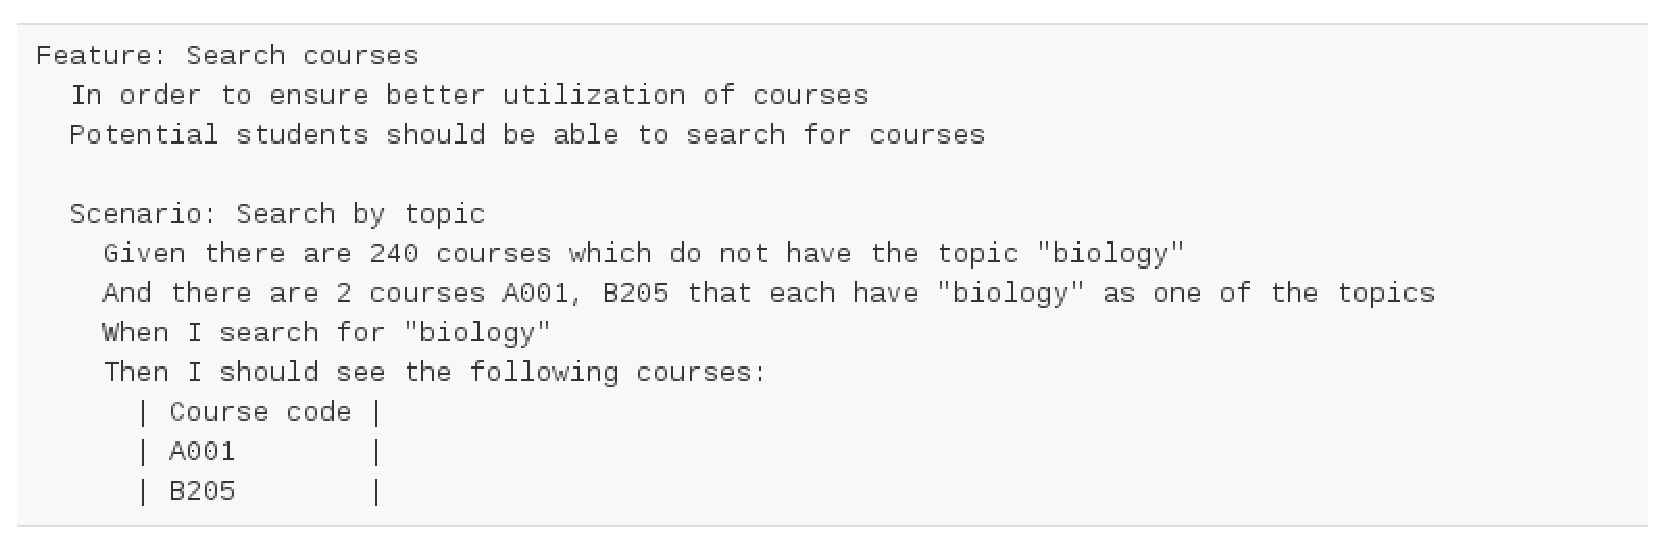
\includegraphics[keepaspectratio=true,scale=0.6]{figuras/cucumber_sample.eps}
	\caption{Exemplo de utilização do cucumber}
	\label{cucumber}
\end{figure}

Apesar do \textbf{cucumber} ter sido desenvolvido para que clientes e usuários
não técnicos possam escrever os as funcionalidades e os cenários em linguagem
próxima à linguagem natural, algumas regras devem ser seguidas uma vez que
a ferramenta precisa traduzir estes textos para uma linguagem que possa ser
interpretada por um computador de forma a automatizar a execução dos testes.
%
Os cenários descritos nesta sessão foram traduzidos para o português e
adaptados para um formato mais adequado para um texto científico.


%------------------------------funcionalidade---------------------------------%
\subsection{\textit{Plugin} Comunidade.UnB}

\subsubsection*{Histórias de usuário}

O \textit{plugin} Comunidade.UnB foi criado para suprir algumas necessidade de
integração de serviços fornecidos pela universidade e a rede de colaboração que
estamos propondo, como a autenticação via base de dados mantida pela universidade.
%
Assim o usuário vai poder ter acesso ao portal de comunidades através dos mesmos
dados utilizados para acessar outros serviços como por exemplo o serviço de
matrícula para alunos ou o serviço de lançamento de notas para professores.

Ao ativar o \textit{plugin}, os campos utilizadas para realizar o \textit{login}
no sistema serão alterados para os mesmo campos utilizados em sistemas da
universidade, matrícula para alunos e prefixo do correio eletrônico para
professores e funcionários técnico-administrativos, e a senha será a mesma.

%TODO adicionar LDAP e CPD nas siglas
Portanto o \textit{plugin} adiciona o campo matrícula e e-mail institucional
(caso o usuário deseje ter manter o campo de e-mail original para seu e-mail
pessoal) além de fazer a integração com o serviço de LDAP no qual o CPD da UnB mantém
os dados dos usuários. Contudo o usuário, durante seu primeiro \textit{login},
escolhe os campos nome de usuário, nome completo e e-mail.

Foi necessário também retirar a funcionalidade de alteração de senha uma vez
que queremos manter a compatibilidade entre o portal de comunidades proposto
e os demais serviços. Desta forma, caso o usuário deseje trocar sua senha 
mesmo deve procurar o CPD e solicitar a alteração.

Até o momento da escrita deste texto, conseguimos autorização para utilizar
apenas a base de dados que contém os dados dos alunos de forma que a
história de usuário e os cenários a seguir levarão em consideração apenas
a utilização do portal de comunidades pelos alunos, mas a funcionalidade
se mantém a mesma para professores e servidores técnico-administrativos que
queiram utilizar o serviço do Comunidade.UnB.

%histórias
\begin{enumerate}

%--------------------------------história-------------------------------------%
\item \underline{Autenticação via LDAP da UnB}

\textbf{Como} um aluno da Universidade Brasília

\textbf{Eu quero} me autenticar na rede através da minha matricula e senha
utilizada em outros sistemas.

\subsubsection*{Cenários de uso:}

%cenários
\begin{enumerate}

%---------------------------------cenário-------------------------------------%
\item \underline{Primeiro acesso}

\textbf{Dado} que sou aluno da UnB

\textbf{E} possuo cadastro ativo na base de dados da UnB

\textbf{E} nunca utilizei o serviço do Comunidade.UnB

\textbf{Quando} eu acessar o portal

\textbf{E} preencher os campos matricula e senha com a matrícula e a senha
fornecidas a mim pela universidade

\textbf{Então} deverei ser direcionado para uma página com o título
"Primeiro Acesso"

\textbf{E} deverei ver os campos "nome de usuário", "nome completo" e
"e-mail pessoal" em vazio.

%---------------------------------cenário-------------------------------------%
\item \underline{Registro}

\textbf{Dado} que sou aluno da UnB

\textbf{E} me encontro na página de primeiro acesso do Comunidade.UnB

\textbf{Quando} eu preencher os campos "nome de usuário",
"nome completo" e "e-mail pessoal" com "daniel.bucher", "Daniel Costa Bucher" e
"daniel.bucher88@gmail.com"

\textbf{E} clicar no botão "Registrar"

\textbf{Então} eu devo ser direcionado para meu perfil

\textbf{E} devo ver a url "<domínio>/daniel.bucher"

\textbf{E} devo ver "Daniel Costa Bucher" abaixo da imagem padrão de perfis
do Noosfero.

%---------------------------------cenário-------------------------------------%

\item \underline{Acesso}

\textbf{Dado} que sou aluno da UnB

\textbf{E} já utilizei o serviço do Comunidade.UnB

\textbf{Quando} eu entrar com minha matricula e senha fornecida pela universidade
nos campos adequados para autenticação

\textbf{E} clicar em entrar

\textbf{Então} eu devo me encontrar \textit{logado} no sistema com a minha conta.

%cenários
\end{enumerate}

%histórias
\end{enumerate}

\subsubsection*{Desenvolvedores responsáveis:}

%desenvolvedores

%TODO adicionar desenvolvedores responsáveis

%desenvolvedores

%------------------------------funcionalidade---------------------------------%
\subsection{Melhorias no \textit{plugin} de sub-organizações}

As histórias de usuários listadas nesta sub-seção dizem respeito a melhorias
no \textit{plugin} de sub-organizações do Noosfero e foram desenvolvidas em
conjunto com a Colivre e a equipe do Portal da Faculdade UnB Gama - FGA.

No Noosfero, uma organização é a abstração de uma entidade que pode assumir
o papel tanto de comunidade quanto de empreendimento. Os cenários de uso das
histórias a seguir foram especificados utilizando comunidades como exemplo,
mas as alterações realizadas afetam da mesma forma a relação entre usuários
e empreendimentos.

%TODO colocar figura da relação de heranças organização -> comunidade/empreendimento

O termo ``organização mãe'' é utilizado para designar uma organização que
possua sub-organizações, também chamadas de organizações filhas. Conforme
descrito acima, uma organização mãe pode ser tanto uma comunidade quanto um
empreendimento.

\subsubsection*{Histórias de usuário:}

%histórias de usuário
\begin{enumerate}

%--------------------------------história-------------------------------------%
\item \underline{Listar organizações `mãe' na lista de organizações de um usuário}

Esta história de usuário está mapeada no ActionItem de número 2825\footnote{\url
{https://noosfero.org/Development/ActionItem2825}}.

\textbf{Como} um usuário

\textbf{Eu quero} visualizar organizações mãe de sub-organizações que faço
parte junto à lista de minhas organizações.

\subsubsection*{Cenários de uso:}

%cenários
\begin{enumerate}

%---------------------------------cenário-------------------------------------%
\item \underline{Ver comunidade `mãe' na página `Gerenciar meus grupos'}

\textbf{Dado} que eu estou logado com a usuário `ze'

\textbf{E} `ze' não é membro do Comunidade.UnB

\textbf{E} `ze' é membro da sub-comunidade de Unb, FGA

\textbf{Quando} eu navegar até a página `Gerenciar meus grupos'
(/myprofile/ze/memberships)

\textbf{Então} eu tenho que ver o Comunidade.UnB listada junto às
demais comunidades que faço parte.

%---------------------------------cenário-------------------------------------%
\item \underline{Ver comunidade `mãe' na página `Comunidades de ze'}

\textbf{Dado} que eu estou logado com a usuário `ze'

\textbf{E} `ze' não é membro do Comunidade.UnB

\textbf{E} `ze' é membro da sub-comunidade de Unb, FGA

\textbf{Quando} eu navegar até a página `Comunidades de ze'
(/profile/ze/communities)

\textbf{Então} eu tenho que ver o Comunidade.UnB listada junto às
demais comunidades que faço parte.

%cenários
\end{enumerate}

%--------------------------------história-------------------------------------%
\item \underline{Bloco de organizações relacionadas}

Esta história de usuário está mapeada no ActionItem de número 2499\footnote{\url
{https://noosfero.org/Development/ActionItem2499}}.

\textbf{Para} ter acesso às organizações relacionadas a uma organização

\textbf{Como} um usuário

\textbf{Eu quero} visualizar um bloco que liste todas as organizações
relacionadas à organização atual.

\subsubsection*{Cenários de uso:}

%cenários
\begin{enumerate}

%---------------------------------cenário-------------------------------------%
\item \underline{Adicionar um bloco de sub-organizações}

\textbf{Dado} que eu estou logado com meu usuário

\textbf{E} meu usuário é administrador da comunidade X

\textbf{Quando} eu navegar até o painel de controle da comunidade X

\textbf{E} eu clicar em "Editar blocos laterais"

\textbf{E} eu clicar em "Adicionar bloco"

\textbf{Então} eu tenho que ver a opção 'Organizações Relacionadas'.

%---------------------------------cenário-------------------------------------%
\item \underline{Listar todas as sub-organizações na organização `mãe'}

\textbf{Dado} que eu estou logado com meu usuário

\textbf{E} meu usuário é membro da comunidade X

\textbf{E} e a comunidade Y é uma sub-comunidade de X

\textbf{E} e o empreendimento Z é um sub-empreendimento de X

\textbf{E} a comunidade X possua um bloco de organizações relacionadas

\textbf{Quando} eu navegar até a página da comunidade X

\textbf{Então} eu tenho que ver um bloco com o título 'Sub organizações'.

\textbf{E} eu tenho que ver um \textit{link} para a sub-comunidade Y neste
bloco

\textbf{E} eu tenho que ver um \textit{link} para o sub-empreendimento Z neste
bloco.

%---------------------------------cenário-------------------------------------%
\item \underline{Listar apenas as sub-comunidades organização `mãe'}

\textbf{Dado} que eu estou logado com meu usuário

\textbf{E} meu usuário é membro da comunidade X

\textbf{E} e a comunidade Y é uma sub-comunidade de X

\textbf{E} e o empreendimento Z é um sub-empreendimento de X

\textbf{E} a comunidade X possua um bloco de organizações relacionadas

\textbf{E} o bloco esteja configurado para mostrar apenas comunidades

\textbf{Quando} eu navegar até a página da comunidade X

\textbf{Então} eu tenho que ver um bloco com o título 'Sub comunidades'.

\textbf{E} eu tenho que ver um \textit{link} para a sub-comunidade Y neste
bloco

\textbf{E} eu não tenho que ver um \textit{link} para o sub-empreendimento Z
neste bloco.

%---------------------------------cenário-------------------------------------%
\item \underline{Visualizar página de sub-organizações de uma organização `mãe'}

\textbf{Dado} que eu estou logado com meu usuário

\textbf{E} meu usuário é membro da comunidade X

\textbf{E} e a comunidade Y é uma sub-comunidade de X

\textbf{E} e o empreendimento Z é um sub-empreendimento de X

\textbf{E} a comunidade X possua um bloco de organizações relacionadas

\textbf{Quando} eu navegar até a página da comunidade X

\textbf{E} eu clicar no link "Ver todos" do bloco de organizações relacionadas

\textbf{Então} eu tenho que ver uma página de sub-organizações

\textbf{E} eu tenho que ver um \textit{link} para a sub-comunidade Y neste
bloco

\textbf{E} eu tenho que ver um \textit{link} para o sub-empreendimento Z
neste bloco.

%---------------------------------cenário-------------------------------------%
\item \underline{Visualizar página de sub-comunidades de uma organização `mãe'}

\textbf{Dado} que eu estou logado com meu usuário

\textbf{E} meu usuário é membro da comunidade X

\textbf{E} e a comunidade Y é uma sub-comunidade de X

\textbf{E} e o empreendimento Z é um sub-empreendimento de X

\textbf{E} a comunidade X possua um bloco de organizações relacionadas

\textbf{E} o bloco esteja configurado para mostrar apenas comunidades

\textbf{Quando} eu navegar até a página da comunidade X

\textbf{E} eu clicar no link "Ver todos" do bloco de organizações relacionadas

\textbf{Então} eu tenho que ver uma página de sub-organizações

\textbf{E} eu tenho que ver um \textit{link} para a sub-comunidade Y neste
bloco

\textbf{E} eu não tenho que ver um \textit{link} para o sub-empreendimento Z
neste bloco.

%---------------------------------cenário-------------------------------------%
\item \underline{Listar todas as organizações `mãe' de uma organização}

\textbf{Dado} que eu estou logado com meu usuário

\textbf{E} meu usuário é membro da comunidade X

\textbf{E} e a comunidade Y é `mãe' de X

\textbf{E} e o empreendimento é `pai' de X

\textbf{E} a comunidade X possua um bloco de organizações relacionadas

\textbf{Quando} eu navegar até a página da comunidade X

\textbf{Então} eu tenho que ver um bloco com o título 'Organizações pais'.

\textbf{E} eu tenho que ver um \textit{link} para a sub-comunidade Y neste
bloco

\textbf{E} eu tenho que ver um \textit{link} para o sub-empreendimento Z neste
bloco.

%cenários
\end{enumerate}

%--------------------------------história-------------------------------------%
\item \underline{Visualização completa nas páginas de organização relacionadas}

\textbf{Como} um usuário

\textbf{Eu quero} visualizar informações sobre as organizações relacionadas nas
páginas de organizações relacionadas

\textbf{Para} me informar sobre elas sem precisar visitar a página de cada uma.

\subsubsection*{Cenários de uso:}

%cenários
\begin{enumerate}

%---------------------------------cenário-------------------------------------%
\item \underline{Visualizar modo completo na página de sub-organizações}

\textbf{Dado} a comunidade X

\textbf{E} a comunidade Y é `filha' de X

\textbf{E} o empreendimento Z é `filho' de X

\textbf{Quando} eu navegar até a página de sub-organizações de X

\textbf{E} eu clicar na opção de visualização completa

\textbf{Então} eu tenho que ver as informações

%cenários
\end{enumerate}

%histórias de usuário
\end{enumerate}

%-----------------------------------------------------------------------------%

\subsubsection*{Desenvolvedores responsáveis:}

Os seguintes colaboradores do Noosfero participaram do desenvolvimento desta
funcionalidade:

%desenvolvedores
\begin{enumerate}

\item Aurélio A. Heckert - Colivre

\item Daniel Bucher - UnB

\item Equipe do Portal FGA - UnB

%desenvolvedores
\end{enumerate}

%------------------------------funcionalidade---------------------------------%
\subsection{\textit{Plugin} de bloco de video}

Esta funcionalidade foi desenvolvido pela equipe do Portal
da FGA e está mapeada no ActionItem de número 2823\footnote{\url{https://
noosfero.org/Development/ActionItem2823}} e consiste em um \textit{plugin}
que adicionar um novo tipo de bloco no Noosfero, o VideoBlock.

Este bloco incorpora vídeos de plataformas externas, atualmente o Vimeo
e o Youtube, dentro de seu conteúdo.

%histórias
\begin{enumerate}

%--------------------------------história-------------------------------------%
\item \underline{Bloco de video}

\textbf{Para} adicionar vídeos em um perfil do Noosfero

\textbf{Como} um usuário

\textbf{Eu quero} ter um bloco em que eu possa adicionar um vídeo de plataformas
como o Youtube\footnote{\url{https://youtube.com}} e o Vimeo\footnote{\url{https://
vimeo.com}}.

\subsubsection*{Cenários de uso:}

%cenários
\begin{enumerate}

%---------------------------------cenário-------------------------------------%
\item \underline{Adicionar bloco}

\textbf{Dado} que estou logado como o usuário `Zé'

\textbf{E} o \textit{plugin} Video esteja atualizado

\textbf{Quando} eu navegar até a página "Editar blocos laterais" do meu perfil

\textbf{E} clicar em "Adicionar bloco"

\textbf{E} selecionar "Bloco de vídeo"

\textbf{E} clicar em "Adicionar"

\textbf{Então} eu devo ver um bloco de vídeo sem conteúdo na área principal.


%---------------------------------cenário-------------------------------------%
\item \underline{Adicionar vídeo do Youtube}

\textbf{Dado} que estou logado como o usuário `Zé'

\textbf{E} possui um bloco de vídeo no meu perfil

\textbf{Quando} eu navegar até a página de "Editar blocos laterais" do meu perfil

\textbf{E} clicar em "Editar" no bloco de vídeo

\textbf{E} adicionar a URL de um video do Youtube

\textbf{E} preencher os campos "Largura" e "Altura" com 536 e 360
respectivamente

\textbf{E} clicar em "Salvar"

\textbf{Então} eu devo ver o vídeo incorporado na área principal do meu
perfil na resolução "536x360".


%---------------------------------cenário-------------------------------------%

\item \underline{Adicionar vídeo do Vimeo}

\textbf{Dado} que estou logado como o usuário `Zé'

\textbf{E} possui um bloco de vídeo no meu perfil

\textbf{Quando} eu navegar até a página de "Editar blocos laterais" do meu perfil

\textbf{E} clicar em "Editar" no bloco de vídeo

\textbf{E} adicionar a URL de um video do Vimeo

\textbf{E} preencher os campos "Largura" e "Altura" com 536 e 360
respectivamente

\textbf{E} clicar em "Salvar"

\textbf{Então} eu devo ver o vídeo incorporado na área principal do meu
perfil na resolução "536x360".

%cenários
\end{enumerate}

%histórias
\end{enumerate}

\subsubsection*{Desenvolvedores responsáveis}

Os seguintes colaboradores do Noosfero participaram do desenvolvimento desta
funcionalidade:

%desenvolvedores
\begin{enumerate}

\item Daniel Bucher - UnB

\item Equipe do Portal FGA - UnB

%desenvolvedores
\end{enumerate}
 
%TODO revisar funcionalidade
%------------------------------funcionalidade---------------------------------%
\subsection{Usabilidade do bloco \textit{links}}

%TODO Dividir em mais de uma user story

Implementar melhorias no Bloco ``Links'', para que fique muito mais intuitivo para um usuário personalizar o seu menu lateral. Incluindo;
- Mover itens por meio de ``Drag and Drop''
- Interface fácil de incluir links para conteúdo próprio.

Implementar melhorias no bloco ``links'' para aumentar a usabilidade:
  - Permitir reorganização de link via ``drag and drop''
  - Interface fácil de inserir links para conteúdo

\subsubsection*{Histórias de usuário}

\begin{enumerate}

%--------------------------------história-------------------------------------%
\item \underline{Mover itens por \textit{Drag and Drop}}

\textbf{Como} um usuário do Noosfero

\textbf{Eu quero} reordenar os items de um bloco de \textit{links} por meio de
\textit{Drag and Drop}.

\subsubsection*{Cenários de uso}

\begin{enumerate}

\item \underline{Arrastar um item}

\textbf{Dado} que eu estou logado com meu usuário

\textbf{E} estou na página de edição de blocos laterais

\textbf{E} eu clico no botão de edição do bloco padrão de links

\textbf{E} eu veja 'Perfil' em cima de 'Galeria de imagens'

\textbf{Quando} arrastar 'Galeria de imagens' para cima de 'Perfil'

\textbf{E} clicar no botão 'Salvar'

\textbf{E} eu for para a página do meu perfil

\textbf{Então} eu tenho que ver 'Galeria de imagens' em cima de 'Perfil'
no bloco de links padrão do perfil.

\end{enumerate}

%--------------------------------história-------------------------------------%
\item \underline{\textit{Auto-complete} ao adicionar novos itens}
%TODO elaborar user story

\end{enumerate}





%-----------------------------------------------------------------------------%

As funcionalidades apresentadas neste capítulo representam as principais
contribuições nas quais houve participação direta de nossa parte. A
funcionalidade de melhoria no \textit{plugin} de sub-organizações
(\ref{feature:sub_organizations}) foi desenvolvida em conjunto com membros
da Colivre, que fariam algumas melhorias no mesmo como parte de um conjunto de
melhorias e novas funcionalidades para o Stoa, a rede de colaboração da USP.
%
No entanto, nós julgamos que seria interessante adicionar algumas melhorias
além do que estava previsto para o Stoa e decidimos colaborar para que fossem
alcançadas.
%
Além das funcionalidades listadas, foram desenvolvidas uma série de outras
funcionalidades em conjunto com a equipe do Portal da FGA de forma a
transmitir o conhecimento adquirido por nós no desenvolvimento do Noosfero
e ajudar a forma uma equipe capacitada a contribuir com o Comunidade.UnB
e com o Noosfero no geral. No momento da escrita deste texto, foram criados
pelo menos 13 \textit{merge-requests}, contando as contribuições deste trabalho
e as contribuições da equipe do Portal da FGA que contaram com nossa contribuição,
diretamente ou indiretamente, dos quais 2 foram aceitos e outros estão em
processo de revisão.

